\documentclass{report}
\usepackage{polski}
\usepackage[utf8]{inputenc}
\usepackage{amsmath}
\usepackage{amsfonts}
\usepackage{amssymb}
\usepackage{graphicx}
\usepackage{listings}
\usepackage{enumerate}
\usepackage{color}

\begin{document}

\chapter{Communication server}
	
	Communication server sprawuje najważniejszą rolę w działaniu całego systemu. Zajmuje się
	przyjmowaniem zadań oraz przydzielaniem zasobów potrzebnych do ich rozwiązania,
	dba o poprawne i bezpieczne przechowywanie wyników i innych obiektów komunikacyjnych.
	Pełni rolę swojego rodzaju pośrednika w komunikacji między innymi elementami klastra.
	
	Communication server ze względu na swoje znaczenie ma możliwość podłączenia dodatkowego
	communication server'a uruchomienia w trybie \textit{backup}, z którym będzie
	prowadzona dodatkowa synchronizacja danych, w celu bezproblemowego działania
	w przypadku utraty jednego z nich.
	
	Dla zwiększenia czytelności przedstawiony zostanie tryb normalny, różnice w trybie
	backup zostaną uwidocznione w osobnym podrozdziale.
	
	
\section{Cykl życia serwera}
	Communication server zaraz po uruchomieniu sprawdza poprawność własnej konfiguracji,
	istnienia niezbędnych zależności (bazy danych). Gdy wszystko przebiegnie pomyślnie
	tworzy dwa wątki - nasłuchujący oraz operacyjny.
	
	Wątek nasłuchujący zajmuje się oczekiwaniem i obsługiwaniem wstępnym nadchodzących 
	komunikatów z innych komponentów klastra obliczeniowego. Konkretne zachowanie zależne
	jest od rodzaju komunikatu, jeżeli otrzymujemy zapytanie o parametry serwera
	odpowiedź finalna jest udzielana od razu, ale jeśli jest to zlecenie podzadania,
	poprawne przyjęcie jest sygnalizowane dopiero po synchronizacji z drugim communication server'em,
	jeśli taki jest ustawiony i dostępny.
	
	Wątek operacyjny zaś, nieustannie (gdy ma taką możliwość) dba o redundancję danych wymieniając 
	się danymi z innym communication server'em będącym w trybie \textit{backup} oraz rozsyła komunikaty 
	przydzielając poszczególne zadania,	ze względu na zachowanie ciągłości synchronizacji ilość 
	przydzielonych zadań w jednym cyklu jest dobierana eksperymentalnie i całkowicie konfigurowalna.
	Co jakiś czas wątek ten sprawdza również obecność wszystkich komponentów i aktualizuje ich listy
	obsługiwanych wtyczek. 
	
	Ogólny diagram aktywności communication server'a można znaleźć na rysunku 
	~\ref{CommunicationServerGeneralActivity}.
	
	\begin{figure}
		\centering
		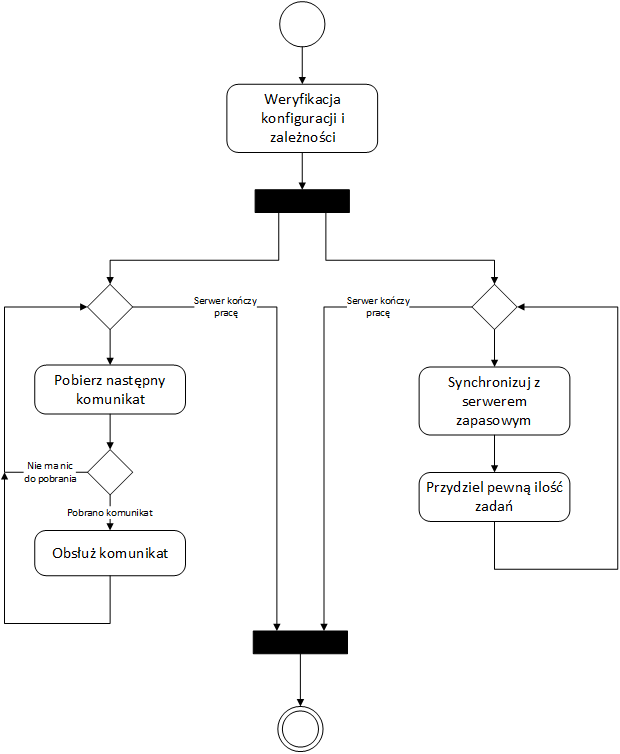
\includegraphics[width=\textwidth]{img/CommunicationServer-General.png}
		\caption{Ogólny diagram aktywności communication server'a}
		\label{CommunicationServerGeneralActivity}
	\end{figure}
	
\section{Cykl życia zadania}

	Dla każdego zadania możemy wyodrębnić kilka jego głównych stanów. Nowo zlecone zadanie
	trafia nieprzetworzone do odpowiedniej kolejki, oczekując na przesłanie do task manager'a
	i podzielenie na łatwiejsze do rozwiązania podproblemy. Po podzieleniu, zadanie czeka na rozwiązanie
	wygenerowanych podzadań, a po ich otrzymaniu wygenerowane jest rozwiązanie, które oczekuje potem na
	pobranie przez użytkownika; lub zgłaszane są dodatkowe podzadania potrzebne do wygenerowania poprawnego
	wyniku.
	
	\begin{figure}[h]
		\centering
		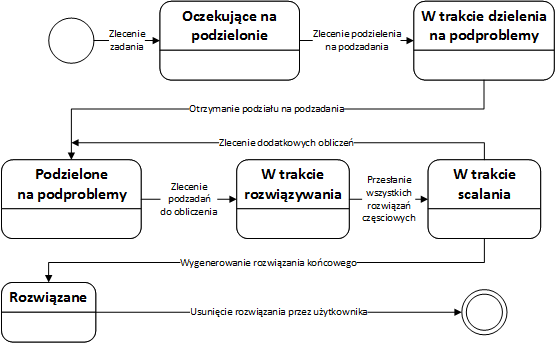
\includegraphics[width=\textwidth]{img/state/Task.png}
		\caption{Diagram stanów zadania}
	\end{figure}
	
\section{Przydzielanie zadań}
	W celu optymalnego przechowywania zleconych przez użytkownika zadań opracowaliśmy
	strukturę ich przechowywania w której główny podział stanowi rodzaj problemu
	(TSP, DVRP itp.), a jego w obrębie znajdują się osobne listy FIFO dla nowo zgłoszonych problemów,
	podproblemów do rozwiązania oraz podproblemów do scalenia. Rodzaj problemu dla przyspieszenia obliczeń
	przechowywuje także informacje o menadżerach zadań i węzłach obliczeniowych, które potrafią
	go obsłużyć. 
	
	Communication server w momencie wyboru zadania filtruje rodzaje problemów w poszukiwaniu takich,
	które są mają oczekujące zadania oraz są rozwiązywalne, czyli posiadają do dyspozycji wolny task manager 
	oraz mają zlecone jakieś zadanie. Spośród tych rodzajów wybieramy zadanie zlecone najwcześniej, by zachować
	oczekiwaną kolejność zajmowania się z zadaniami.
	
	Przy przydzielaniu podzadań dla poszczególnych computational node'ów postępujemy analogicznie.
	
	Rozwiązania podzadań odsyłamy do task manager'a w celu scalenia po otrzymaniu ich wszystkich. Menadżer
	po analizie odpowiedzi może zdecydować o wygenerowaniu rozwiązania końcowego lub zlecić podzadania dodatkowe
	i odłożyć końcową odpowiedź na termin późniejszy. 
	
	\begin{figure}[h]
		\centering
		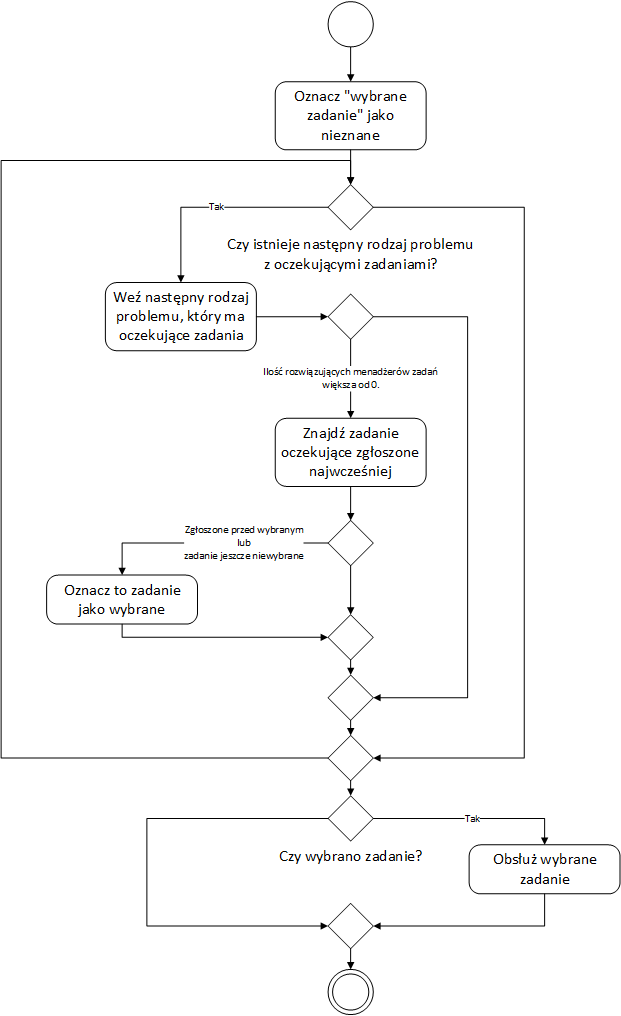
\includegraphics[width=\textwidth]{img/CommunicationServer-SelectTask.png}
		\caption{Wybór zadania przez communication server}
	\end{figure}
	
	Nie należy zapominać również o zadaniach które zostały zlecone, ale z jakichś powodów
	nie zostały wykonane w oczekiwanym czasie. Takie zadania wracają do kolejki i czekają na
	ponowne przydzielenie.
	
\section{Tryb backup}
	Serwer w trybie backup zachowuje się bardzo podobnie do serwera w trybie normalnym.
	Najistotniejszą różnicą jest to, że stara się on być jedynie nośnikiem danych
	i nie wykonywać żadnych operacji na dostępnych zasobach. W przypadku próby zlecenia
	mu zadania podczas gdy nie jest on jedynym serwerem przekierowuje je do głównego communication server'a.
	Jeżeli zaś communication server nie odpowiada, przejmuje jego obowiązki.
	W momencie przywrócenia sprawności serwera głównego, synchronizują się one w normalnym
	trybie, a serwer główny staje się w pełni operacyjny.
	
\section{Synchronizacja między serwerami}
	Obiekty w czasie stworzenia i zapisania do jednej z baz danych oznaczane są jako obiekty
	do synchronizacji i są wymieniane między serwerami w następnym cyklu w formie wiadomości
	synchronizacyjnej. Podobnie dzieje się z zmodyfikowanymi obiektami (modyfikowane
	mogą być jedynie pola z datą przydzielenia pracy i informacją o zleceniobiorcy).
	Po otrzymaniu potwierdzenia odebrania są oznaczone jako zsynchronizowane. Jeśli
	potwierdzenie nie zostanie otrzymane, wykonywana jest retransmisja po odpowiednim
	czasie oczekiwania.
	
\end{document}